\documentclass[12pt]{exam}
\usepackage{tikz}
\usepackage[colorlinks=true]{hyperref}

\begin{document}

\noindent

\firstpageheader{}{\textbf{\huge{Exam}}\\\textnormal{Gnew}}{}


\begin{questions}

\question Determine $x$.
\[9^{2x-1} - 9^{2x-2} = 1944\]
\vspace{6cm}

\question Determine values of $a$, $b$, and $c$ that satisfy both equations.

\[ab + c = 2050\]
\[a + bc = 2051\]

\newpage

\question Calculate the perimter of the figure below.

\begin{center}
    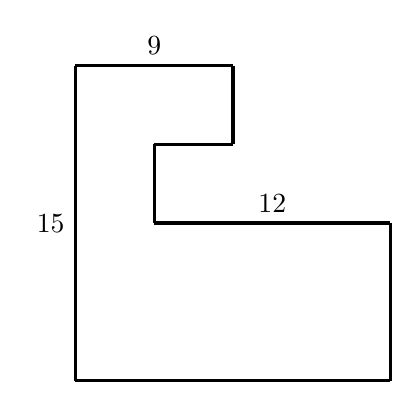
\begin{tikzpicture}
		\draw[very thick] (0,0) -- node[left] {$15$} (0,4);
		\draw[very thick] (0,4) -- node[above] {$9$} (2,4);
        \draw[very thick] (2,4) -- (2,3);
        \draw[very thick] (2,3) -- (1,3);
        \draw[very thick] (1,3) -- (1,2);
		\draw[very thick] (1,2) -- node[above] {$12$} (4,2);
        \draw[very thick] (4,2) -- (4,0);
        \draw[very thick] (4,0) -- (0,0);
    \end{tikzpicture}
\end{center}

\vspace{6cm}

\question Determine $\frac{dy}{dx}$, then find an equation for the tangent line at $x = 3$.

\[12y - x^{2}y^{3} - 16x = 0\]

\newpage

\question Bob received a score of 138 on an IQ test. His wife scored 134. If they had a child, which of the following most accurately predicts his score?

\begin{choices}
	\choice 120
	\choice 136
	\choice 142
	\choice 100
\end{choices}
\vspace{1cm}

\question A and B are found to correlate with r = 0.23. This implies a \fillin[][1in] relationship between A and B.

\begin{choices}
	\choice weak negative
	\choice strong negative
	\choice weak positive
	\choice strong positive
\end{choices}
\vspace{1cm}

\question Determine $\displaystyle\lim_{x\to 0} \frac{7x-\sin(x)}{x^{2}+\sin(3x)}$.
\vspace{6cm}

\newpage

\question Determine $\displaystyle\lim_{x\to 0} \frac{-2x^{4}+6x^{2}-4x}{x^{2}-2x}$.
\vspace{20cm}

DM your answers to \href{https://discord.com/users/1007410169145212958}{Gnew\#7805}. The first person to get a 75 or above will recieve sloppy toppy.

\end{questions}

\end{document}
